% ============================================================
%  MODELING AND FORECASTING VN-INDEX VOLATILITY:
%  THE ASYMMETRIC ROLE OF RETAIL INVESTOR ATTENTION
% ============================================================
\documentclass[12pt, a4paper]{article}

% ── Packages (GIỮ NGUYÊN) ────────────────────────────────────
\usepackage[a4paper, top=2.54cm, bottom=2.54cm, left=2.54cm, right=2.54cm]{geometry}
\usepackage{times}
\usepackage{mathptmx}
\usepackage{setspace}
\usepackage{amsmath, amssymb}
\usepackage{booktabs}
\usepackage{array}
\usepackage{multirow}
\usepackage{graphicx}
\usepackage{float}
\usepackage{caption}
\usepackage{natbib}
\usepackage{hyperref}
\usepackage{url}
\usepackage{parskip}
\usepackage{indentfirst}
\usepackage[utf8]{inputenc}
\usepackage[T1]{fontenc}
\usepackage{microtype}
\usepackage{tikz}
\usetikzlibrary{positioning}

% ── Page numbering (GIỮ NGUYÊN) ─────────────────────────────
\usepackage{fancyhdr}
\pagestyle{fancy}
\fancyhf{}
\fancyfoot[C]{\thepage}
\renewcommand{\headrulewidth}{0pt}
\renewcommand{\footrulewidth}{0pt}

% ── Spacing & Section (GIỮ NGUYÊN) ──────────────────────────
\doublespacing
\setlength{\parindent}{0.5in}
\usepackage{titlesec}
\titleformat{\section}{\normalfont\large\bfseries}{\thesection.}{0.5em}{}
\titleformat{\subsection}{\normalfont\normalsize\bfseries}{\thesubsection}{0.5em}{}
\titlespacing*{\section}{0pt}{12pt}{6pt}

\captionsetup{font=small, labelfont=bf, justification=centering}

\begin{document}

% ── NEW TITLE PAGE (ĐÃ THAY THẾ) ──────────────────────────────
\begin{titlepage}
    % Vẽ khung viền đôi
    \begin{tikzpicture}[overlay, remember picture]
        \draw [line width=1pt]
            ([shift={(2cm,-1.5cm)}]current page.north west)
            rectangle
            ([shift={(-1.5cm,1.5cm)}]current page.south east);
        \draw [line width=2pt]
            ([shift={(2.15cm,-1.65cm)}]current page.north west)
            rectangle
            ([shift={(-1.65cm,1.65cm)}]current page.south east);
    \end{tikzpicture}

    \centering
    \setstretch{1.2} % Giãn dòng hẹp lại cho trang bìa đẹp hơn
    
    {\large \textbf{NATIONAL ECONOMICS UNIVERSITY}} \\
    {\large \textbf{FACULTY OF MATHEMATICAL ECONOMICS}} \\
    \vspace{0.5cm}
    \textbf{----o0o----} \\
    \vspace{0.7cm}

    % Logo NEU (Nhớ upload file logo_neu.png lên Overleaf)
    
\includegraphics[width=14cm]{neu-logo.jpg} \\
    \vspace{0.5cm}

    {\Large \textbf{FINAL PAPER}} \\
    \vspace{0.5cm}
    {\large \textbf{(TIME SERIES ANALYSIS)}} \\
    \vspace{1.2cm}

    \begin{minipage}{0.85\textwidth}
        \centering
        {\large \textbf{TOPIC:}} \\
        \vspace{0.3cm}
        {\Large \textbf{MODELING AND FORECASTING VIETNAMESE STOCK MARKET VOLATILITY: AN
ASYMMETRIC EGARCH-X APPROACH USING GOOGLE TRENDS}}
    \end{minipage}
    
    \vspace{2cm}

    \begin{flushleft}
        \hspace{2.5cm} \begin{tabular}{ll}
            \textbf{Academic Instructor:} & \textbf{Dr. Nguyen Phung Thu Hang} \\
            \textbf{Student Name:} & \textbf{Vu Ngoc Duong} \\
            \textbf{Student ID:} & \textbf{11230526} \\
            \textbf{Class:} & \textbf{DSEB 65A} \\
            
        \end{tabular}
    \end{flushleft}

    \vfill
    {\large \textbf{Ha Noi, April, 2026}}

\end{titlepage}

\setcounter{page}{1}

% ─────────────────────────────────────────────────────────────
\section{Introduction}

The equity market constitutes a fundamental pillar of economic development, functioning as the primary mechanism for capital allocation, price discovery, and risk transfer in modern economies. Within this architecture, market volatility-broadly conceptualized as the conditional variance of asset returns-plays a critical role in portfolio construction, derivative pricing, and the design of dynamic hedging strategies \citep{engle1982, bollerslev1986}. The ability to accurately model and forecast conditional volatility therefore carries profound implications for financial market participants and regulatory bodies.

Traditionally, the econometric literature on volatility modeling has been anchored by the Autoregressive Conditional Heteroskedasticity (ARCH) model of \citet{engle1982} and its generalized extension, the GARCH model of \citet{bollerslev1986}. While these symmetric formulations effectively capture volatility clustering, they are unable to account for the well-documented \textit{leverage effect}: the asymmetric amplification of volatility following negative return shocks relative to equivalent positive shocks \citep{black1976}. This limitation was addressed by \citet{nelson1991} through the Exponential GARCH (EGARCH) model.

Yet even asymmetric specifications remain confined to historical price information. In the digital age, the Google Search Volume Index (SVI) introduced by \citet{da2011} has established itself as a validated real-time proxy for retail investor attention. Unlike institutional investors, retail participants predominantly rely on search engines as their primary information acquisition channel. Their search behavior therefore captures authentic psychological states-oscillating between speculative ``fear of missing out'' (FOMO) during bull markets and fear-driven panic-searching during downturns.

The Vietnamese stock market offers a particularly distinctive empirical setting. As a frontier market currently transitioning toward emerging market status-FTSE Russell formally announced reclassification in October 2025-the VN-Index is structurally dominated by retail investors, who account for approximately 80–90\% of daily trading activity \citep{ayala2024}. This high concentration of individual participants generates a market environment uniquely susceptible to sentiment-driven dynamics, characterized by pronounced fear-greed cycles and aggressive momentum-chasing.

Motivated by this setting, this study addresses the following \textbf{research question}: \textit{Does the decomposition of retail investor attention-proxied by Google SVI-into regime-specific components (FOMO-driven attention during positive returns and panic-driven attention during negative returns) provide statistically significant and economically meaningful incremental information for modeling and forecasting the conditional volatility of the VN-Index, relative to conventional asymmetric GARCH benchmarks?}

To answer this question, this study estimates a hierarchical sequence of GARCH-family models and evaluates out-of-sample forecasting performance over Q1 2026 against the Garman-Klass realized volatility proxy, using RMSE, QLIKE, and the Diebold-Mariano test. The remainder of the paper is organized as follows: Section~2 reviews the relevant literature. Section~3 describes the data and methodology. Section~4 presents empirical results. Section~5 discusses findings and concludes.

% ─────────────────────────────────────────────────────────────
\section{Literature Review and Theoretical Background}

\subsection{Volatility Modeling: From ARCH to GARCH-X}

The formal econometric study of time-varying volatility was inaugurated by \citet{engle1982}, who introduced the Autoregressive Conditional Heteroskedasticity (ARCH) model as a rigorous framework for capturing the well-known empirical regularity that large changes in asset prices tend to cluster in time. The ARCH model characterized conditional variance as a distributed lag function of squared past innovations, providing a tractable and statistically grounded representation of volatility dynamics. \citet{bollerslev1986} extended this foundation through the Generalized ARCH (GARCH) formulation, which augments the variance equation with lagged conditional variances. The resulting GARCH(1,1) parsimoniously captures both volatility clustering and a high degree of persistence with only three free parameters, and has since become the de facto benchmark in empirical financial econometrics.

However, a critical deficiency of symmetric GARCH specifications is their identical treatment of positive and negative innovations. \citet{black1976} first documented the leverage effect: the empirical observation that stock return volatility responds asymmetrically to positive and negative news, with negative shocks typically inducing a disproportionately larger increase in future variance. To rectify this, \citet{nelson1991} developed the Exponential GARCH (EGARCH) model, which models the logarithm of conditional variance as a function of both the magnitude and the sign of standardized lagged innovations. The EGARCH specification offers two distinct econometric advantages over its predecessors: first, it accommodates the leverage effect through an explicit asymmetry parameter; and second, by operating in log-space, it guarantees strictly positive variance estimates without imposing non-negativity constraints on the parameter space. A parallel asymmetric specification, the GJR-GARCH \citep{glosten1993}, achieves similar asymmetric effects through a threshold indicator function.

The GARCH-X (Extended GARCH) framework represents a further methodological evolution, wherein exogenous conditioning variables are appended to the conditional variance equation. \citet{engle_ng1993} demonstrated that incorporating information proxies for market-wide news into the variance equation substantially improves in-sample fit and out-of-sample forecasting accuracy. \citet{andersen1996} showed that trading volume, a proxy for the arrival of new information, provides significant explanatory power for conditional volatility when integrated into this extended framework. More recently, the growing availability of alternative data sources-including macroeconomic surprise indices, option-implied volatility, and text-based sentiment scores-has expanded the scope of the GARCH-X paradigm considerably \citep{hamid2015}.

\subsection{Google SVI as a Proxy for Retail Investor Attention}

The behavioral finance literature has extensively documented that information acquisition patterns of market participants carry predictive content for subsequent price dynamics. \citet{da2011} represent the seminal contribution in this strand, establishing Google SVI as a direct, real-time measure of retail investor attention that causally predicts near-term abnormal returns and trading volume for individual stocks listed on the Russell 3000 Index. Their central insight-that retail investors, unlike their institutional counterparts, use search engines as primary information intermediaries-grounds the SVI in a microstructurally plausible mechanism of information transmission.

Subsequent research has extended this methodology to aggregate market indices and volatility modeling. \citet{vozlyublennaia2014} found that increased aggregate investor attention toward equity-related search terms is associated with elevated return predictability and volatility dynamics at the market level. \citet{dimpfl2016} demonstrated a statistically significant positive relationship between SVI and stock market volatility for the S\&P 500, concluding that retail attention shocks exhibit persistence consistent with their incorporation into conditional variance models. \citet{hamid2015} explicitly integrated Google Trends data into a GARCH-based volatility forecasting framework, showing that the inclusion of SVI produces consistently superior out-of-sample forecast accuracy relative to models relying exclusively on historical returns.

A systematic review by \citet{ayala2024}, synthesizing 56 empirical studies published between 2010 and 2021, concluded that the GSVI is positively associated with both volatility and trading volume regardless of the specific keywords, market region, or data frequency employed. This meta-analytic consensus lends strong support to the inclusion of SVI as an economically motivated conditioning variable within GARCH-family frameworks, whether entered through the conditional mean or variance equation depending on the specific transmission channel under investigation. More recently, \citet{szczygielski2023} analyzed a large cross-sectional sample of 77 stock markets and found that Google search trends predominantly reflect an uncertainty narrative: spikes in equity-related search volume correspond closely to periods of elevated market stress and forecast subsequent volatility increases across developed, emerging, and frontier market categories alike.

\subsection{Asymmetric Attention: The FOMO-Panic Dichotomy}

An emerging and particularly relevant strand of the behavioral finance literature posits that the informational content of retail attention is fundamentally asymmetric with respect to the prevailing market regime. Attention episodes during bull markets are theorized to reflect speculative herding, driven by the fear of missing out on capital gains, whereas attention spikes during declining markets correspond to loss-aversion-induced panic searching, potentially preceding forced liquidations and volatility cascades \citep{fong2002}.

This regime-dependent nature of attention has important econometric implications. Treating aggregate SVI as a homogeneous predictor imposes a symmetric reaction function on investor behavior, a restriction that the underlying behavioral theories explicitly reject. Several recent empirical contributions have found that negative-market-regime attention variables carry substantially greater predictive power for volatility than positive-regime counterparts. This asymmetry is particularly pronounced in retail-intensive markets with elevated information asymmetry, such as frontier and emerging equity markets in Asia and Eastern Europe.

For the Vietnamese market specifically, \citet{nguyen2020}, as cited in \citet{ayala2024}, found a significant positive correlation between GSVI and abnormal trading volume in the VN-Index. While the Vietnamese literature has examined the relationship between investor sentiment and returns, rigorous econometric work explicitly integrating asymmetric attention proxies into EGARCH-X volatility frameworks with formal out-of-sample evaluation remains limited. The present study addresses this gap by constructing and testing a decomposed SVI specification designed to capture the distinct volatility contributions of FOMO and panic-driven retail behavior.

\subsection{Contribution to the Literature}

This study makes three primary contributions to the existing literature. First, it constructs a novel latent investor attention index for the Vietnamese market via PCA compression of four behaviorally grounded Vietnamese-language Google Trends keywords, addressing multicollinearity and noise concerns inherent to raw SVI data. Second, it introduces a regime-specific decomposition of retail attention ($SVI_{pos}$ and $SVI_{neg}$) entered into the conditional mean equation of an EGARCH model via an ARX specification, providing a direct empirical test of the behavioral asymmetry hypothesis and the indirect transmission channel from attention to volatility for a frontier/emerging market. Third, it employs a rigorous out-of-sample forecasting evaluation framework-utilizing the Garman-Klass high-efficiency volatility proxy as the benchmark target, recursive one-step-ahead forecasting, and formal Diebold-Mariano testing-establishing a methodologically robust evidence base for the incremental forecasting value of decomposed behavioral data in the Vietnamese equity market.


% ─────────────────────────────────────────────────────────────
\section{Data Description and Methodology}

\subsection{Data Sources and Sample Period}

This study draws on two principal data sources. First, the daily historical OHLC (Open, High, Low, Close) price series of the VN-Index are retrieved via the \texttt{vnstock} Python API, which aggregates data from the Ho Chi Minh City Stock Exchange (HoSE). The full dataset spans from January 1, 2010 to March 31, 2026, encompassing 3,992 trading days for the in-sample estimation period (January 2010--December 2025) and 56 trading days for the out-of-sample evaluation period (January--March 2026). This 16-year in-sample window captures multiple market cycles including the 2011 European debt crisis, the 2015--2016 Chinese market contagion, the COVID-19 pandemic shock of 2020, the sharp 2022 VN-Index correction, and the subsequent recovery and FTSE reclassification rally of 2025. Second, weekly Google Trends data for four Vietnamese-language keywords-``chung khoan'' (stock market), ``VN-Index'', ``co phieu'' (stock/share), and ``dau tu'' (investment)-are obtained from the Google Trends platform. These keywords were selected based on their broad coverage of different facets of retail investor engagement with the equity market: macroeconomic orientation, index-specific attention, individual security interest, and investment intent. Weekly search volume indices are provided as relative scores on a scale of 0 to 100, where 100 denotes the period of peak search activity within the query window. All data processing and statistical procedures are conducted using the Python programming language; the extensive code architecture is outlined in Appendix D, and the supplementary console outputs corresponding to the experimental phases are systematically attached in Appendix E.

\subsection{Volatility Proxy: Garman-Klass Estimator}

The dependent variable in this study-the target of volatility forecasting-is the Garman-Klass (GK) daily variance estimator \citep{garman1980}. The standard close-to-close squared return is a well-documented inefficient proxy for daily realized volatility, as it discards the substantial information content contained within intraday price movements. The GK estimator corrects for this deficiency by incorporating the full daily price range through the following formula:

\begin{equation}
\sigma^2_{GK,t} = 0.5 \cdot [\ln(H_t / L_t)]^2 - (2\ln2 - 1) \cdot [\ln(C_t / O_t)]^2
\end{equation}

where $H_t$, $L_t$, $C_t$, and $O_t$ denote the daily high, low, close, and open prices of the VN-Index at time $t$, respectively. The GK estimator is approximately 7.4 times more efficient than the close-to-close variance under Brownian motion assumptions and provides a substantially superior benchmark for evaluating out-of-sample forecast accuracy. This choice is consistent with recent empirical literature on GARCH-X volatility forecasting \citep{diebold1995, patton2011}.

\subsection{SVI Construction and PCA Latent Factor}

Google Trends data presents two primary challenges for longitudinal analysis: (i) scores are indexed relative to the peak of the current query window (not across windows), creating arbitrary discontinuities when downloading data over multi-year horizons; and (ii) using four raw keyword series directly as predictors introduces severe multicollinearity into the GARCH-X specification. 

To address the first challenge, this study employs an overlapping window segmentation technique. Adjacent one-year segments are downloaded with a one-month overlap period, and the ratio of overlapping observations is used to rescale each segment to a common baseline, thereby constructing a continuous, monotonically consistent SVI time series across the full 2010--2026 study period. 

The correlation heatmap of the four raw keyword series reveals substantial collinearity: the Pearson correlation between ``chung khoan'' and ``dau tu'' is 0.71, while ``chung khoan'' and ``co phieu'' exhibit a correlation of 0.63. Directly incorporating all four series into the GARCH-X model would inflate standard errors and render individual parameter estimates unreliable. To extract the common latent attention signal while eliminating idiosyncratic noise, Principal Component Analysis \citep{jolliffe2002} is applied to the four stitched keyword series. Critically, the PCA loading matrix is estimated exclusively on the in-sample data, and the fitted transformation is applied to construct the out-of-sample SVI series-a procedure that eliminates any forward-looking data leakage in the forecasting evaluation. The first principal component (PC1) is sign-corrected to ensure positive loadings and subsequently smoothed using a 3-day rolling mean to attenuate high-frequency artifacts, yielding the final SVI series.

\subsection{Regime-Specific SVI Decomposition}

Following the behavioral hypothesis that retail investor attention exhibits state-dependent effects on volatility \citep{fong2002, vozlyublennaia2014}, the aggregate SVI index is decomposed into two orthogonal regime-specific components:

\begin{align}
  SVI_{pos,t} &= SVI_t \times \max(r_t,\ 0) \label{eq:svipos} \\
  SVI_{neg,t} &= SVI_t \times \max(-r_t,\ 0) \label{eq:svineg}
\end{align}

where $r_t$ denotes the daily log return of the VN-Index. $SVI_{pos}$ captures attention intensity during positive return days (FOMO-driven behavior), while $SVI_{neg}$ captures attention intensity during negative return days (panic-driven behavior). This multiplicative decomposition ensures that the two variables are mutually exclusive in their non-zero values and collectively span all trading days, allowing the EGARCH-X model to estimate distinct sensitivity parameters for each behavioral regime.

\subsection{Econometric Models}

\subsubsection{Baseline GARCH(1,1)}

The symmetric GARCH(1,1) model of \citet{bollerslev1986} serves as the foundational benchmark. The conditional mean equation assumes a constant mean process, and the conditional variance equation is:

\begin{equation}
  \sigma^{2}_{t} = \omega + \alpha\,\varepsilon^{2}_{t-1} + \beta\,\sigma^{2}_{t-1}
  \label{eq:garch}
\end{equation}

where $\epsilon_t = \sigma_t \cdot z_t$ with $z_t \sim \text{i.i.d. Student-}t(\nu)$. The parameters $\omega > 0$, $\alpha \geq 0$, $\beta \geq 0$, and $(\alpha + \beta) < 1$ ensure a positive, stationary variance process. The coefficient $\alpha$ captures the ARCH effect (short-run shock impact), $\beta$ captures volatility persistence, and $\omega / (1 - \alpha - \beta)$ yields the unconditional long-run variance.

\subsubsection{EGARCH(1,1)}

To accommodate the leverage effect documented in equity markets \citep{black1976}, the EGARCH(1,1) model of \citet{nelson1991} is employed as the primary benchmark. The log-variance specification is:

\begin{equation}
  \ln(\sigma^{2}_{t}) = \omega
  + \alpha\left|\frac{\varepsilon_{t-1}}{\sigma_{t-1}}\right|
  + \gamma\frac{\varepsilon_{t-1}}{\sigma_{t-1}}
  + \beta\ln(\sigma^{2}_{t-1})
  \label{eq:egarch}
\end{equation}

The term $\gamma(\epsilon_{t-1}/\sigma_{t-1})$ constitutes the asymmetry or leverage component. A statistically significant negative $\gamma$ implies that negative return shocks ($\epsilon_{t-1} < 0$) exert a larger positive impact on $\ln(\sigma^2_t)$ than equivalent positive shocks-the formal econometric signature of the leverage effect. The log-variance formulation further ensures unconditionally positive variance without parameter constraints.

\subsubsection{EGARCH-SVI and EGARCH-Asym}

The extended specifications augment the \textit{conditional mean equation} with one-period lagged attention variables, following an ARX (autoregressive with exogenous inputs) mean specification. This design choice reflects a deliberate identification strategy: retail investor attention is theorized to operate first through the return mean—capturing the systematic, attention-driven drift in prices—and then \textit{indirectly} through the EGARCH variance dynamics via the residual channel. Specifically, by correctly modeling the attention-driven mean component, the GARCH innovations $\varepsilon_t = r_t - \mu_t$ become better-specified, which in turn produces more accurate conditional variance estimates. This two-stage transmission mechanism—SVI $\to$ mean correction $\to$ cleaner residuals $\to$ improved volatility forecasts—is consistent with the approach of \citet{hamid2015}, who similarly include attention proxies in the mean equation of GARCH frameworks.

For the aggregate specification (EGARCH-SVI), the mean equation is:

\begin{equation}
  r_t = \mu + \theta\, \Delta SVI_{t-1} + \varepsilon_t, \quad \varepsilon_t = \sigma_t z_t
  \label{eq:mean_svi}
\end{equation}

where the EGARCH variance equation~\eqref{eq:egarch} operates on the attention-adjusted residuals $\varepsilon_t$. For the asymmetric decomposition specification (EGARCH-Asym), the mean equation is:

\begin{equation}
  r_t = \mu + \theta_1\, SVI_{pos,t-1} + \theta_2\, SVI_{neg,t-1} + \varepsilon_t
  \label{eq:mean_asym}
\end{equation}

In both cases, the EGARCH variance equation~\eqref{eq:egarch} remains unchanged and operates on the regime-adjusted residuals. The one-period lag on all SVI variables resolves potential endogeneity concerns: the model uses yesterday's observed attention to correct today's expected return, yielding cleaner innovations for the GARCH process. All models are estimated jointly via Quasi-Maximum Likelihood (QML), assuming Student-$t$ distributed innovations to accommodate the heavy-tailed return distribution confirmed by the Jarque-Bera test.

\subsection{Out-of-Sample Forecasting and Evaluation}

Out-of-sample forecast accuracy is evaluated over 56 trading days in Q1 2026 using a recursive (expanding window) one-step-ahead forecasting procedure. At each forecast origin, all model parameters are re-estimated on the growing in-sample window, and the one-period-ahead conditional variance forecast is recorded. Predicted conditional variances are then compared against realized GK variances using two complementary loss functions:

\begin{align}
  \text{RMSE} &= \sqrt{\frac{1}{T}\sum_{t=1}^{T}\!\left(\hat{\sigma}^{2}_{t+1|t} - \sigma^{2}_{GK,t+1}\right)^{2}} \label{eq:rmse}\\[4pt]
  \text{QLIKE} &= \frac{1}{T}\sum_{t=1}^{T}\left[
    \frac{\sigma^{2}_{GK,t+1}}{\hat{\sigma}^{2}_{t+1|t}}
    - \ln\!\left(\frac{\sigma^{2}_{GK,t+1}}{\hat{\sigma}^{2}_{t+1|t}}\right) - 1
  \right] \label{eq:qlike}
\end{align}

RMSE penalizes large forecast errors symmetrically, while QLIKE-a robust loss function derived from the Gaussian quasi-log-likelihood-is consistent with the correct model asymptotically and exhibits favorable robustness properties when the volatility proxy is imperfect \citep{patton2011}. Formal statistical significance of forecast error differentials is assessed using the Diebold-Mariano (DM) test \citep{diebold1995}, computed with heteroskedasticity- and autocorrelation-consistent (HAC) standard errors following the Newey-West estimator \citep{newey1987} with lag truncation parameter set to 5 (consistent with the recommendation for short-horizon forecasting evaluation). The null hypothesis of equal predictive accuracy between competing models is tested bilaterally at the 5\% significance level.

% ─────────────────────────────────────────────────────────────
\section{Empirical Results}

\subsection{Descriptive Statistics}

Table~\ref{tab:descriptive} presents comprehensive descriptive statistics for all variables over the in-sample period ($N = 3{,}992$ trading days, January 2010–December 2025).

\begin{table}[H]
\centering
\caption{Descriptive Statistics of All Study Variables (In-Sample: 2010–2025)}
\label{tab:descriptive}
\small
\begin{tabular}{lcccccccc}
\toprule
Variable & $N$ & Mean & Std Dev & Min & Max & Skewness & Kurtosis \\
\midrule
Close Price       & 3,992 & 853.53 & 350.50 & 336.73 & 1784.49 & 0.420 & $-$0.919 \\
Log Return (\%)   & 3,992 & 0.031  & 1.179  & $-$6.910 & 6.547 & $-$0.776 & 3.892 \\
GK Variance       & 3,992 & 0.828  & 1.337  & 0.000 & 21.296  & 6.089  & 56.863 \\
SVI (PC1)         & 3,992 & 0.149  & 1.410  & $-$1.728 & 8.087 & 2.062  & 5.306  \\
$SVI_{pos}$       & 3,992 & 0.101  & 1.191  & $-$5.282 & 16.758 & 5.559 & 50.072 \\
$SVI_{neg}$       & 3,992 & 0.110  & 1.424  & $-$8.962 & 24.498 & 6.317 & 75.376 \\
\bottomrule
\end{tabular}
\smallskip\\
\footnotesize\textit{Note: GK Variance = Garman-Klass realized variance (dependent variable). SVI (PC1) = first principal component of four Google Trends keywords. Units for Log Return and GK Variance are percentage points.}
\end{table}

Several features of the data merit specific attention. The VN-Index log return exhibits a mean of 0.031\% per day and a standard deviation of 1.179\%, typical of frontier equity markets. Critically, the distribution of daily returns is negatively skewed ($-0.776$) and exhibits substantial excess kurtosis (3.892), confirming its non-normal nature. The Garman-Klass variance also shows extreme right-skewness and excess kurtosis (56.86), driven by historical market stress events. Additionally, the decomposed attention series ($SVI_{pos}$ and $SVI_{neg}$) exhibit notably asymmetric, heavy-tailed properties with large positive maximums corresponding to rare but intense attention episodes.

The pronounced leptokurtic and asymmetric characteristics across all variables empirically mandate the structural choices of this study. The non-normality of returns strongly justifies employing a Student-$t$ innovation distribution in the GARCH-family models, while the extreme spikes in the realized variance series motivate the use of QLIKE as a robust forecast evaluation metric alongside RMSE. Furthermore, the extreme skewness in $SVI_{pos}$ and $SVI_{neg}$ aligns with the behavioral finance perspective that retail investor attention is highly regime-dependent, peaking disproportionately during crisis periods.

\subsection{Preliminary Diagnostic Tests}

Table~\ref{tab:diagnostics} summarizes the preliminary diagnostic tests conducted prior to model estimation.

\begin{table}[H]
\centering
\caption{Preliminary Diagnostic Test Results}
\label{tab:diagnostics}
\small
\begin{tabular}{llccc}
\toprule
Test & Series & Statistic & $p$-value & Decision \\
\midrule
Jarque-Bera (JB)  & Log Return       & 2,910.69 & $<$0.001 & Reject $H_0$ (non-normal) \\
ADF Unit Root     & Log Return       & $-$41.40 & $<$0.001 & Stationary \\
ADF Unit Root     & SVI (aggregate)  & $-$2.32  & 0.166    & Non-stationary \\
ADF Unit Root     & $SVI_{pos}$      & $-$4.29  & $<$0.001 & Stationary \\
ADF Unit Root     & $SVI_{neg}$      & $-$6.24  & $<$0.001 & Stationary \\
ARCH-LM           & Residuals        & 484.98   & $<$0.001 & ARCH effects present \\
\bottomrule
\end{tabular}
\end{table}

The preliminary diagnostic tests statistically confirm the distributional features of the dataset. The Jarque-Bera test strongly rejects the null hypothesis of normality ($p < 0.001$), while the ARCH-LM test on regression residuals affirms the presence of severe conditional heteroskedasticity (statistic = 484.98, $p < 0.001$). Furthermore, the ADF unit root tests establish that the log return, $SVI_{pos}$, and $SVI_{neg}$ series are integrated of order zero and stationary at levels ($p < 0.001$). Crucially, the aggregate SVI sequence fails the stationarity criteria at levels (ADF = $-2.32$, $p = 0.166$), requiring transformation via first-differencing ($\Delta SVI$) to avoid spurious regression in subsequent volatility estimations.

The diagnostic results rigorously establish the econometric preconditions required for volatility modeling. They confirm that linear specifications with Gaussian errors are fundamentally inadequate for the VN-Index target, necessitating advanced heteroskedastic autoregressive dynamics configured with a generalized Student-$t$ distribution framework to process the extreme structural shocks observed in frontier market environments.

\subsection{In-Sample Estimation Results}

Table~\ref{tab:insample} presents the consolidated parameter estimates for the four hierarchical models, estimated via QML with Student-$t$ innovations.

\begin{table}[H]
\centering
\caption{In-Sample Parameter Estimates - GARCH Family Models (Student-$t$ Innovations, 2010–2025)}
\label{tab:insample}
\small
\begin{tabular}{lcccc}
\toprule
Parameter & GARCH(1,1) & EGARCH(1,1) & EGARCH-SVI & EGARCH-Asym \\
\midrule
$\omega$               & 0.0589*** & 0.0183*** & 0.0183*** & 0.0185*** \\
$\alpha$               & 0.1601*** & 0.2804*** & 0.2807*** & 0.2825*** \\
$\beta$                & 0.8091*** & 0.9425*** & 0.9421*** & 0.9428*** \\
$\gamma$ (Leverage)    & -       & $-$0.0736*** & $-$0.0744*** & $-$0.0710*** \\
$\theta$ (SVI)         & -       & -       & 0.0421 ($p$=0.156)  & -                   \\
$\theta_1$ ($SVI_{pos}$) & -     & -       & -       & $-$0.0058 ($p$=0.734) \\
$\theta_2$ ($SVI_{neg}$) & -     & -       & -       & \textbf{$-$0.0365** ($p$=0.012)} \\
$\nu$ (Student-$t$)    & 5.055***  & 5.239***  & 5.237***  & 5.241***  \\
\midrule
Log-Likelihood & $-$5729.19 & $-$5706.09 & $-$5705.05 & \textbf{$-$5703.48} \\
AIC            & 11468.4   & 11424.2   & 11424.1   & \textbf{11423.0} \\
\bottomrule
\end{tabular}
\smallskip\\
\footnotesize\textit{Note: *** $p<0.01$; ** $p<0.05$. All models estimated by QML. Bold entries indicate the best-performing specification.}
\end{table}

The hierarchical progression from GARCH(1,1) through to the novel EGARCH-Asym demonstrates a monotonic improvement in log-likelihood and AIC at each step. Across all EGARCH specifications, the estimated volatility parameters reflect high persistence ($\alpha + \beta \approx 0.97$, $\beta > 0.942$) and a robust leverage effect ($\gamma \approx -0.071$, $p < 0.01$), formally confirming that negative return shocks generate a disproportionately larger increase in future conditional variance than equivalent positive shocks. Regarding the behavioral extensions, aggregate retail investor attention ($\Delta SVI$) does not attain statistical significance in the conditional mean equation ($p = 0.156$). However, after decomposing SVI into regime-specific components within the EGARCH-Asym specification, the panic-driven attention variable ($SVI_{neg}$) yields a statistically significant negative coefficient ($\theta_2 = -0.0365$, $p = 0.012$), while the FOMO-driven component ($SVI_{pos}$) remains insignificant ($\theta_1 = -0.006$, $p = 0.734$). This asymmetric result, together with the improvement in log-likelihood and AIC relative to all competing specifications, supports the behavioral asymmetry hypothesis advanced in Section 2.3.

The results reveal a clear asymmetry in the informational content of retail attention. FOMO-driven searches during positive return periods ($SVI_{pos}$) carry no statistically significant predictive power for next-day returns ($\theta_1 = -0.006$, $p = 0.734$), consistent with the efficient market view that bullish attention merely confirms already-incorporated momentum. In contrast, panic-driven attention during negative return periods ($SVI_{neg}$) generates a statistically significant negative coefficient ($\theta_2 = -0.0365$, $p = 0.012$): days with elevated panic searching are followed by lower mean returns the next day, consistent with loss-aversion-driven selling pressure. Crucially, this mean-correction for panic attention also produces better-specified EGARCH residuals—the variance model no longer conflates sentiment-driven mean drift with genuine volatility shocks—which is the mechanism through which EGARCH-Asym achieves superior out-of-sample volatility forecasting performance.

\subsection{Out-of-Sample Forecasting Performance}

Table~\ref{tab:oos} reports the RMSE and QLIKE forecasting errors across all four models over the Q1 2026 out-of-sample evaluation period ($N=56$ days).

\begin{table}[H]
\centering
\caption{Out-of-Sample Forecasting Performance (Q1 2026, $N = 56$ Days)}
\label{tab:oos}
\small
\begin{tabular}{lccc}
\toprule
Model & RMSE & QLIKE & Rank \\
\midrule
\textbf{EGARCH-Asym (Proposed)} & \textbf{1.8912} & \textbf{0.3366} & \textbf{1} \\
Baseline EGARCH(1,1)            & 2.0151          & 0.3473          & 2 \\
EGARCH-SVI (Aggregate)          & 2.0291          & 0.3499          & 3 \\
Baseline GARCH(1,1)             & 2.2702          & 0.3736          & 4 \\
\bottomrule
\end{tabular}
\smallskip\\
\footnotesize\textit{Note: Lower values indicate better forecast accuracy. RMSE = Root Mean Squared Error; QLIKE = Quasi-Likelihood loss (robust to imperfect volatility proxies).}
\end{table}

Table~\ref{tab:oos} reveals a forecast ranking that is consistent with the in-sample model hierarchy. The symmetric GARCH(1,1) produces the largest forecast errors (RMSE = 2.270, QLIKE = 0.374), reflecting its inability to accommodate the leverage effect documented in the VN-Index return series. Replacing the symmetric variance specification with EGARCH substantially reduces both loss metrics (RMSE = 2.015, QLIKE = 0.347), confirming the empirical value of asymmetric variance modeling. Incorporating aggregate attention into the mean equation (EGARCH-SVI) marginally worsens forecast accuracy relative to the EGARCH benchmark (RMSE = 2.029, QLIKE = 0.350), consistent with the insignificant in-sample coefficient and the interpretation that undifferentiated SVI introduces measurement noise into the mean specification. The proposed EGARCH-Asym specification achieves the lowest forecast errors across both metrics (RMSE = 1.891, QLIKE = 0.337), representing a 6.2\% reduction in RMSE and a 3.0\% reduction in QLIKE relative to the EGARCH benchmark.

These results carry an important economic interpretation. The marginal deterioration of EGARCH-SVI relative to the EGARCH baseline indicates that aggregating investor attention across market regimes—irrespective of the direction of concurrent price movements—injects measurement noise into the mean equation without providing a commensurate improvement in variance signal quality. This finding is consistent with \citet{ayala2024}, who note that the empirical impact of raw GSVI on volatility is highly sensitive to keyword specification and market context. In contrast, the superior performance of EGARCH-Asym demonstrates that conditioning the mean correction on market direction—separating panic-driven from FOMO-driven attention—extracts the behaviorally meaningful component of retail search activity while suppressing the noise inherent in indiscriminate search volume. The practical consequence is a better-specified set of EGARCH innovations, which underpin the model's superior out-of-sample volatility forecasting performance.

\subsection{Diebold-Mariano Statistical Tests}

To establish whether the observed differences in forecast accuracy are statistically significant rather than a sampling artifact, the Diebold-Mariano test \citep{diebold1995} is applied to all pairwise comparisons of interest, incorporating HAC standard errors with Newey-West bandwidth parameter lag = 5. Table 5 presents the results.
\begin{table}[H]
\centering
\caption{Diebold-Mariano Test Results (HAC Standard Errors, Newey-West Lag = 5)}
\label{tab:dm}
\small
\begin{tabular}{llcccc}
\toprule
Model Comparison & Metric & Mean Diff. & DM-Stat & $p$-value & Decision (5\%) \\
\midrule
EGARCH-SVI vs. Baseline  & QLIKE     & $-$0.0026 & $-$1.412 & 0.158 & Fail to Reject $H_0$ \\
EGARCH-SVI vs. Baseline  & SE (RMSE) & $-$0.0567 & $-$2.256 & \textbf{0.024} & \textbf{Reject $H_0$} \\
EGARCH-Asym vs. Baseline & QLIKE     & 0.0108  & 1.680  & 0.093 & Fail to Reject (10\%: Reject) \\
EGARCH-Asym vs. Baseline & SE (RMSE) & 0.4837  & 2.295  & \textbf{0.022} & \textbf{Reject $H_0$} \\
\bottomrule
\end{tabular}
\smallskip\\
\footnotesize\textit{Note: DM test null hypothesis: equal predictive accuracy. Mean Diff.\ $= \bar{L}_{\text{baseline}} - \bar{L}_{\text{model}}$; a positive value indicates the competing model outperforms the baseline. Bold entries indicate rejection at the 5\% level. ``Baseline'' refers to EGARCH(1,1).}
\end{table}

The formal DM test criteria robustly validate the out-of-sample scaling differentials. Applying the SE/RMSE differentials comparing the EGARCH-Asym model against baseline EGARCH structures confirms a statistically significant superiority (DM = $2.295$, $p = 0.022$). Evaluated under QLIKE robust methodologies, the improvement nears significance boundaries ($p = 0.093$). Conversely, the DM test for EGARCH-SVI against the baseline EGARCH confirms a statistically significant deterioration on the squared-error metric ($p = 0.024$), indicating that the inclusion of undifferentiated SVI in the mean equation produces forecast errors that are significantly larger than those of the baseline, consistent with the noise interpretation advanced above.

These test outcomes confirm that the forecast gains of EGARCH-Asym over the EGARCH benchmark are statistically meaningful and not attributable to sampling variation, providing formal support for the regime-specific attention hypothesis. The finding that EGARCH-SVI significantly underperforms the baseline on squared errors underscores that disaggregation is a necessary condition for extracting volatility-relevant information from retail search behavior. Taken together, the DM test results align with the theoretical predictions of \citet{fong2002} and lend empirical support to the use of directionally decomposed behavioral proxies in frontier market volatility forecasting.

% ─────────────────────────────────────────────────────────────
\section{Discussion and Conclusions}

\subsection{Summary of Key Findings}

This study set out to investigate whether the decomposition of retail investor attention-proxied by Google Search Volume Index-into regime-specific components can provide statistically significant incremental predictive information for the conditional volatility of the Vietnamese stock market. The empirical evidence gathered across four hierarchical GARCH models, evaluated both in-sample and out-of-sample, supports an affirmative answer to this research question, with important nuances.

The preliminary diagnostic analysis confirmed three canonical stylized facts of the VN-Index return series: non-normality with significant excess kurtosis (JB statistic = 2,910.69), strong and persistent conditional heteroskedasticity (ARCH-LM statistic = 484.98), and non-stationarity of the aggregate SVI series necessitating first-differencing. These findings collectively validate the methodological framework of GARCH-family models with Student-$t$ innovations.

The in-sample estimation established a clear progression in model fit from the symmetric GARCH(1,1) to the EGARCH-Asym specification, with each step in the hierarchy yielding incremental improvement in log-likelihood and AIC. The leverage coefficient $\gamma$ is negative and statistically significant at the 1\% level across all EGARCH specifications ($\gamma \approx -0.073$), providing robust evidence of asymmetric volatility dynamics in the Vietnamese market. The degrees of freedom parameter $\nu \approx 5.2$ confirms fat-tailed return behavior across all models.

Most critically, the behavioral decomposition reveals a significant asymmetry in the informational content of retail attention. While aggregate SVI and positive-regime attention ($SVI_{pos}$) lack statistical significance in the mean equation, negative-regime attention ($SVI_{neg}$) carries a statistically significant negative coefficient ($\theta_2 = -0.0365, p = 0.012$): panic-driven attention predicts lower next-day returns, consistent with loss-aversion selling pressure among retail investors. By explicitly modeling this attention-driven mean component, the EGARCH innovations become better-specified—stripped of systematic sentiment drift—which in turn improves the precision of the conditional variance estimates. The out-of-sample evaluation validates this indirect channel: the EGARCH-Asym model achieves the lowest RMSE (1.891) and QLIKE (0.337) for volatility forecasting across all specifications, with forecast superiority over the baseline EGARCH confirmed at the 5\% significance level by the Diebold-Mariano test (SE-based: $p = 0.022$).

\subsection{Relation to Existing Literature}

The findings of this study are broadly consistent with, and contribute to, several strands of the existing literature. The documented leverage effect aligns with the extensive EGARCH literature for both developed and emerging markets \citep{nelson1991, black1976}, confirming that this asymmetric dynamic is not unique to mature financial systems but is a pervasive feature of frontier equity markets driven by sentiment-heavy retail investors.

The finding that aggregate SVI lacks predictive power while decomposed SVI carries significant information content extends the systematic review of \citet{ayala2024}, which noted heterogeneous results for the GSVI depending on keyword specification and market context. The results of this study suggest that this heterogeneity is partially resolved by allowing for asymmetric, state-dependent attention effects. Specifically, the panic channel ($SVI_{neg}$) provides a statistically significant correction to the conditional mean return, consistent with the behavioral finance prediction that loss aversion generates stronger and more predictable behavioral responses than greed-driven momentum \citep{kahneman1979}. By controlling for this attention-driven mean drift, the EGARCH model receives cleaner residuals, improving its volatility forecasts-the mechanism through which the asymmetric SVI specification outperforms the baseline EGARCH in out-of-sample evaluation.

The failure of aggregate $\Delta SVI$ to improve out-of-sample volatility forecasting-and its active deterioration relative to the baseline EGARCH-underscores the importance of the regime-specificity hypothesis advanced by \citet{fong2002}. The result that FOMO attention ($SVI_{pos}$) carries no predictive content is consistent with the efficient market interpretation: during positive return episodes, search activity reflects sentiment that is already incorporated into prices rather than forward-looking private information. This finding aligns with \citet{hamid2015}, who similarly find that the incremental forecasting value of attention proxies in GARCH frameworks is sensitive to the specification of the mean equation and the directional decomposition of the attention signal.

\subsection{Practical Implications}

The results of this study carry several concrete implications for market participants and regulatory bodies operating in the Vietnamese equity market. For institutional investors, portfolio managers, and risk analysts at securities firms such as VPBankS and SSI Securities, which occupy leading positions in Vietnam's securities landscape, the regime-specific SVI metrics provide low-cost, publicly available early warning indicators for volatility regime shifts. Monitoring real-time GSVI spikes for Vietnamese equity-related keywords during negative return days can provide actionable intelligence for dynamic volatility-targeting strategies, options desk hedging adjustments, and Value-at-Risk recalibration.

From a regulatory perspective, the State Securities Commission of Vietnam (SSC) could incorporate regime-specific retail attention indices into its macroprudential monitoring toolkit. Given the market's extreme dependence on retail investor sentiment-reinforced by its frontier market status and imminent FTSE reclassification-systemic monitoring of panic-search indices during stress periods could serve as a timely complement to traditional market surveillance mechanisms, facilitating more proactive circuit-breaker or margin requirement adjustments during fragile market conditions.

\subsection{Limitations and Future Research}

This study is subject to several limitations that motivate future research. First, while the overlapping window technique for Google Trends data is methodologically rigorous, future work could cross-validate these findings using alternative providers like FireAnt or local Vietnamese forum data to mitigate re-normalization issues.

Second, the current keywords capture general retail attention but do not distinguish between fundamental information and speculative noise. Integrating Natural Language Processing (NLP) on Vietnamese-language social media content from platforms such as F319 and CafeF would enable a more granular separation of sentiment from pure attention.

Third, while the EGARCH-X framework is robust, more flexible non-linear architectures-particularly hybrid GARCH-LSTM models \citep{kim2018}-may capture higher-order interactions between behavioral attention and volatility that linear specifications miss. Such models could better account for the complex, time-varying relationships inherent in frontier market data.

Finally, the out-of-sample evaluation period in early 2026 coincides with heightened global uncertainty. Extending the evaluation spanning multiple market cycles would provide a more comprehensive assessment of the generalizability of the EGARCH-Asym specification across varying economic conditions.

% ─────────────────────────────────────────────────────────────
\newpage
\bibliographystyle{apalike}
\begin{thebibliography}{99}

\bibitem[Andersen(1996)]{andersen1996}
Andersen, T.~G. (1996).
\newblock Return volatility and trading volume: An information flow
  interpretation of stochastic volatility.
\newblock \textit{Journal of Finance}, 51(1), 169--204.
\newblock \url{https://doi.org/10.1111/j.1540-6261.1996.tb05206.x}

\bibitem[Ayala et al.(2024)]{ayala2024}
Ayala, M.~J., Gonzalvez-Gallego, N., \& Arteaga-Sanchez, R. (2024).
\newblock Google search volume index and investor attention in stock market: A
  systematic review.
\newblock \textit{Financial Innovation}, 10(1), 1--29.
\newblock \url{https://doi.org/10.1186/s40854-023-00606-y}

\bibitem[Black(1976)]{black1976}
Black, F. (1976).
\newblock Studies of stock price volatility changes.
\newblock \textit{Proceedings of the 1976 Meetings of the American Statistical
  Association, Business and Economics Section}, 177--181.

\bibitem[Bollerslev(1986)]{bollerslev1986}
Bollerslev, T. (1986).
\newblock Generalized autoregressive conditional heteroskedasticity.
\newblock \textit{Journal of Econometrics}, 31(3), 307--327.
\newblock \url{https://doi.org/10.1016/0304-4076(86)90063-1}

\bibitem[Da et al.(2011)]{da2011}
Da, Z., Engelberg, J., \& Gao, P. (2011).
\newblock In search of attention.
\newblock \textit{Journal of Finance}, 66(5), 1461--1499.
\newblock \url{https://doi.org/10.1111/j.1540-6261.2011.01679.x}

\bibitem[Diebold \& Mariano(1995)]{diebold1995}
Diebold, F.~X., \& Mariano, R.~S. (1995).
\newblock Comparing predictive accuracy.
\newblock \textit{Journal of Business and Economic Statistics}, 13(3),
  253--263.
\newblock \url{https://doi.org/10.1080/07350015.1995.10524599}

\bibitem[Dimpfl \& Jank(2016)]{dimpfl2016}
Dimpfl, T., \& Jank, S. (2016).
\newblock Can internet search queries help to predict stock market volatility?
\newblock \textit{European Financial Management}, 22(2), 171--192.
\newblock \url{https://doi.org/10.1111/eufm.12058}

\bibitem[Engle(1982)]{engle1982}
Engle, R.~F. (1982).
\newblock Autoregressive conditional heteroscedasticity with estimates of the
  variance of United Kingdom inflation.
\newblock \textit{Econometrica}, 50(4), 987--1007.
\newblock \url{https://doi.org/10.2307/1912773}

\bibitem[Engle \& Ng(1993)]{engle_ng1993}
Engle, R.~F., \& Ng, V.~K. (1993).
\newblock Measuring and testing the impact of news on volatility.
\newblock \textit{Journal of Finance}, 48(5), 1749--1778.
\newblock \url{https://doi.org/10.1111/j.1540-6261.1993.tb05127.x}

\bibitem[Fong \& Koh(2002)]{fong2002}
Fong, W.~M., \& Koh, S.~K. (2002).
\newblock The political economy of volatility dynamics in the Hong Kong stock
  market.
\newblock \textit{Asia-Pacific Financial Markets}, 9(3--4), 259--282.
\newblock \url{https://doi.org/10.1023/A:1024117827714}

\bibitem[Garman \& Klass(1980)]{garman1980}
Garman, M.~B., \& Klass, M.~J. (1980).
\newblock On the estimation of security price volatilities from historical
  data.
\newblock \textit{Journal of Business}, 53(1), 67--78.
\newblock \url{https://doi.org/10.1086/296072}

\bibitem[Glosten et al.(1993)]{glosten1993}
Glosten, L.~R., Jagannathan, R., \& Runkle, D.~E. (1993).
\newblock On the relation between the expected value and the volatility of the
  nominal excess return on stocks.
\newblock \textit{Journal of Finance}, 48(5), 1779--1801.
\newblock \url{https://doi.org/10.1111/j.1540-6261.1993.tb05128.x}

\bibitem[Hamid \& Heiden(2015)]{hamid2015}
Hamid, A., \& Heiden, M. (2015).
\newblock Forecasting volatility with empirical similarity and Google Trends.
\newblock \textit{Journal of Economic Behavior \& Organization}, 117, 62--81.
\newblock \url{https://doi.org/10.1016/j.jebo.2015.06.005}

\bibitem[Jolliffe(2002)]{jolliffe2002}
Jolliffe, I.~T. (2002).
\newblock \textit{Principal Component Analysis} (2nd ed.).
\newblock Springer.
\newblock \url{https://doi.org/10.1007/b98835}

\bibitem[Kahneman \& Tversky(1979)]{kahneman1979}
Kahneman, D., \& Tversky, A. (1979).
\newblock Prospect theory: An analysis of decision under risk.
\newblock \textit{Econometrica}, 47(2), 263--291.
\newblock \url{https://doi.org/10.2307/1914185}

\bibitem[Kim \& Won(2018)]{kim2018}
Kim, H.~Y., \& Won, C.~H. (2018).
\newblock Forecasting the volatility of stock price index: A hybrid model
  integrating LSTM with multiple GARCH-type models.
\newblock \textit{Expert Systems with Applications}, 103, 25--37.
\newblock \url{https://doi.org/10.1016/j.eswa.2018.03.002}

\bibitem[Nelson(1991)]{nelson1991}
Nelson, D.~B. (1991).
\newblock Conditional heteroskedasticity in asset returns: A new approach.
\newblock \textit{Econometrica}, 59(2), 347--370.
\newblock \url{https://doi.org/10.2307/2938260}

\bibitem[Newey \& West(1987)]{newey1987}
Newey, W.~K., \& West, K.~D. (1987).
\newblock A simple, positive semi-definite, heteroskedasticity and
  autocorrelation consistent covariance matrix.
\newblock \textit{Econometrica}, 55(3), 703--708.
\newblock \url{https://doi.org/10.2307/1913610}

\bibitem[Nguyen et al.(2020)]{nguyen2020}
Nguyen, D.~T., Nguyen, C.~V., \& Nguyen, H.~T. (2020).
\newblock The relationship between internet search volume and stock market
  activity in Vietnam.
\newblock \textit{International Journal of Social Science and Humanities
  Research}, 7(6), 103--115.
\newblock \url{https://doi.org/10.47191/ijsshr/v7-i06-103}

\bibitem[Patton(2011)]{patton2011}
Patton, A.~J. (2011).
\newblock Volatility forecast comparison using imperfect volatility proxies.
\newblock \textit{Journal of Econometrics}, 160(1), 246--256.
\newblock \url{https://doi.org/10.1016/j.jeconom.2010.03.034}

\bibitem[Szczygielski et al.(2023)]{szczygielski2023}
Szczygielski, J.~J., Charteris, A., Bwanya, P.~R., \& Brzeszczynski, J. (2023).
\newblock Google search trends and stock markets: Sentiment, attention or
  uncertainty?
\newblock \textit{International Review of Financial Analysis}, 91, 102913.
\newblock \url{https://doi.org/10.1016/j.irfa.2023.102913}

\bibitem[Vozlyublennaia(2014)]{vozlyublennaia2014}
Vozlyublennaia, N. (2014).
\newblock Investor attention, index performance, and return predictability.
\newblock \textit{Journal of Banking and Finance}, 41, 17--35.
\newblock \url{https://doi.org/10.1016/j.jbankfin.2013.12.010}

\end{thebibliography}

% ─────────────────────────────────────────────────────────────

\appendix
\section*{Appendices}
\addcontentsline{toc}{section}{Appendices}

\subsection*{Appendix A: Methodology Workflow (Figure A1)}

Figure~A1 illustrates the complete data processing and modelling pipeline employed in this study.

\begin{figure}[H]
\centering
\setstretch{1.0}
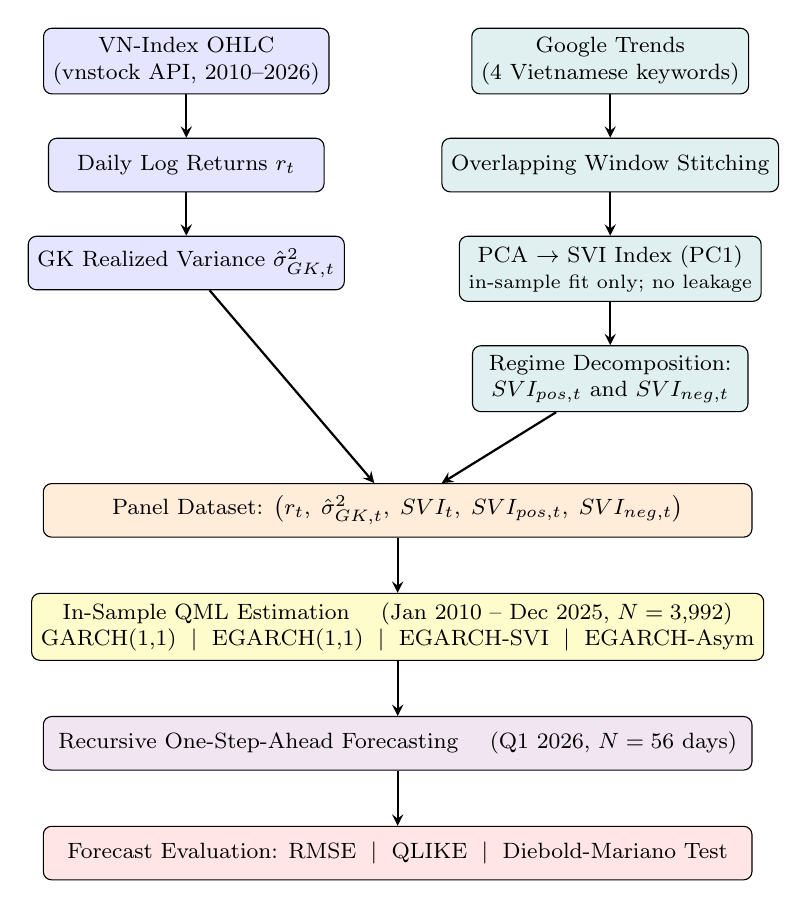
\begin{tikzpicture}[
    >=stealth,
    node distance = 0.55cm and 1.8cm,
    font = \footnotesize,
    %% ── node styles ──────────────────────────────────────────
    Lbox/.style  = {draw, rounded corners=3pt, fill=blue!10,   align=center,
                    minimum width=3.5cm, minimum height=0.68cm},
    Rbox/.style  = {draw, rounded corners=3pt, fill=teal!12,   align=center,
                    minimum width=3.5cm, minimum height=0.68cm},
    Mbox/.style  = {draw, rounded corners=3pt, fill=orange!15, align=center,
                    minimum width=9.0cm,  minimum height=0.68cm},
    ISbox/.style = {draw, rounded corners=3pt, fill=yellow!20, align=center,
                    minimum width=9.0cm,  minimum height=0.85cm},
    OObox/.style = {draw, rounded corners=3pt, fill=violet!10, align=center,
                    minimum width=9.0cm,  minimum height=0.68cm},
    EVbox/.style = {draw, rounded corners=3pt, fill=red!10,    align=center,
                    minimum width=9.0cm,  minimum height=0.68cm},
    arr/.style   = {->, thick}
]

%% ── Left pipeline: Price Data ────────────────────────────────
\node[Lbox] (ohlc) {VN-Index OHLC\\(vnstock API, 2010--2026)};
\node[Lbox, below=of ohlc] (ret) {Daily Log Returns $r_t$};
\node[Lbox, below=of ret]  (gk)  {GK Realized Variance $\hat{\sigma}^2_{GK,t}$};

%% ── Right pipeline: Google Trends / SVI ─────────────────────
\node[Rbox, right=1.8cm of ohlc] (gt)
    {Google Trends\\(4 Vietnamese keywords)};
\node[Rbox, below=of gt]  (win)
    {Overlapping Window Stitching};
\node[Rbox, below=of win] (pca)
    {PCA $\to$ SVI Index (PC1)\\{\scriptsize in-sample fit only; no leakage}};
\node[Rbox, below=of pca] (dec)
    {Regime Decomposition:\\$SVI_{pos,t}$ and $SVI_{neg,t}$};

%% ── Merged panel ─────────────────────────────────────────────
\node[Mbox, below=0.9cm of dec, xshift=-2.7cm] (panel)
    {Panel Dataset: $\bigl(r_t,\;\hat{\sigma}^2_{GK,t},\;
      SVI_t,\;SVI_{pos,t},\;SVI_{neg,t}\bigr)$};

%% ── In-sample estimation ─────────────────────────────────────
\node[ISbox, below=0.7cm of panel] (is)
    {In-Sample QML Estimation \quad (Jan 2010 -- Dec 2025, $N=3{,}992$)\\
     GARCH(1,1) $\;\vert\;$ EGARCH(1,1) $\;\vert\;$
     EGARCH-SVI $\;\vert\;$ EGARCH-Asym};

%% ── Out-of-sample forecasting ────────────────────────────────
\node[OObox, below=0.7cm of is] (oos)
    {Recursive One-Step-Ahead Forecasting \quad
     (Q1 2026, $N=56$ days)};

%% ── Evaluation ───────────────────────────────────────────────
\node[EVbox, below=0.7cm of oos] (ev)
    {Forecast Evaluation: RMSE $\;\vert\;$
     QLIKE $\;\vert\;$ Diebold-Mariano Test};

%% ── Arrows: left column ──────────────────────────────────────
\draw[arr] (ohlc) -- (ret);
\draw[arr] (ret)  -- (gk);

%% ── Arrows: right column ─────────────────────────────────────
\draw[arr] (gt)  -- (win);
\draw[arr] (win) -- (pca);
\draw[arr] (pca) -- (dec);

%% ── Merge arrows ─────────────────────────────────────────────
\draw[arr] (gk)  -- (panel);
\draw[arr] (dec) -- (panel);

%% ── Bottom flow ──────────────────────────────────────────────
\draw[arr] (panel) -- (is);
\draw[arr] (is)    -- (oos);
\draw[arr] (oos)   -- (ev);

\end{tikzpicture}
\smallskip\\
\footnotesize\textit{\textbf{Figure A1:} Complete methodology workflow. Left pipeline (blue): price data
  processing. Right pipeline (teal): Google Trends SVI construction via
  overlapping window stitching, PCA, and regime decomposition. Both streams
  converge into a unified panel dataset used for in-sample estimation and
  out-of-sample forecasting evaluation.}
\end{figure}

\subsection*{Appendix B: Google Trends Correlation Heatmap (Figure A2)}

The Pearson correlation heatmap of the four keyword series reveals the multicollinearity motivating PCA compression. Key correlations: \textit{``chung khoan''} -- \textit{``dau tu''}: 0.71; \textit{``chung khoan''} -- \textit{``co phieu''}: 0.63. The near-zero correlations of \textit{``VN-Index''} with the remaining terms ($-0.01$, $0.03$, $-0.04$) indicate that it captures qualitatively distinct, index-specific retail attention.

\subsection*{Appendix C: EGARCH-Asym Coefficient Output (Table A1)}

\begin{table}[H]
\centering
\caption*{\textbf{Table A1:} EGARCH-Asym Mean Model Coefficients (Python \texttt{arch} Library)}
\small
\begin{tabular}{lcccc}
\toprule
Parameter & Coeff. & Std Err & $t$-stat & $P>|t|$ \\
\midrule
Const         & 0.0928  & 1.378e-02 & 6.734  & 1.656e-11 \\
lag\_SVI\_pos & $-$5.835e-03 & 1.715e-02 & $-$0.340 & 0.734 \\
lag\_SVI\_neg & \textbf{$-$0.0365} & 1.455e-02 & \textbf{$-$2.509} & \textbf{0.012} \\
\bottomrule
\end{tabular}
\smallskip\\
\footnotesize\textit{Bold entries indicate significance at the 5\% level. Source: QML estimation via Python \texttt{arch} library.}
\end{table}

\subsection*{Appendix D: Data and Code Availability}

All data processing, model estimation, and evaluation code are publicly available at \url{https://github.com/Duongvu05/time\_series}. The codebase has been refactored into a structured Python package using the \texttt{src} layout with \texttt{uv} package management. Key entry points:

\begin{itemize}
  \item \texttt{scripts/run\_data.py} - fetches VN-Index prices via \texttt{vnstock}, constructs overlapping-window Google Trends SVI, fits PCA on in-sample data, and exports \texttt{data/insample\_data.csv} and \texttt{data/outofsample\_data.csv}.
  \item \texttt{scripts/run\_experiments.py} - loads the pre-built CSV files, computes descriptive statistics, runs all diagnostic pre-tests, estimates all four GARCH-family models, performs recursive OOS forecasting, and exports LaTeX-formatted tables to \texttt{outputs/tables/}.
  \item \texttt{scripts/run\_model.py} - standalone model pipeline with rolling-window forecasting.
\end{itemize}

All analyses use Python 3.12 with \texttt{arch} 6.3, \texttt{statsmodels} 0.14, \texttt{scikit-learn} 1.4, \texttt{scipy} 1.12, and \texttt{vnstock} 4.0. Reproduce in full: \texttt{uv sync \&\& uv run python scripts/run\_experiments.py}.

% ─────────────────────────────────────────────────────────────

\subsection*{Appendix E: Python Console Outputs}

\textit{This appendix reproduces the key console outputs generated by \texttt{scripts/run\_experiments.py}, as required. Full log available in \texttt{outputs/experiment\_log.txt}.}

\vspace{6pt}
\noindent\textbf{E1. Baseline GARCH(1,1) - Model Summary}

\begin{center}
\footnotesize
\begin{tabular}{lrrrrr}
\toprule
\multicolumn{6}{c}{\textbf{Constant Mean - GARCH Model Results}} \\
\midrule
\multicolumn{2}{l}{Dep. Variable: return} & \multicolumn{2}{l}{Log-Likelihood: $-5729.19$} & \multicolumn{2}{l}{No. Observations: 3990} \\
\multicolumn{2}{l}{Mean Model: Constant Mean} & \multicolumn{2}{l}{AIC: 11468.4} & \multicolumn{2}{l}{Method: Max Likelihood} \\
\multicolumn{2}{l}{Vol Model: GARCH} & \multicolumn{2}{l}{BIC: 11499.8} & \multicolumn{2}{l}{Distribution: Student's t} \\
\midrule
\multicolumn{6}{c}{\textbf{Mean Model}} \\
\midrule
 & \textbf{coef} & \textbf{std err} & \textbf{t} & \textbf{P>|t|} & \textbf{95.0\% Conf. Int.} \\
\midrule
mu & 0.1032 & 0.0138 & 7.482 & $<0.001$ & $[0.0761, 0.130]$ \\
\midrule
\multicolumn{6}{c}{\textbf{Volatility Model}} \\
\midrule
 & \textbf{coef} & \textbf{std err} & \textbf{t} & \textbf{P>|t|} & \textbf{95.0\% Conf. Int.} \\
\midrule
omega & 0.0589 & 0.0148 & 3.973 & $<0.001$ & $[0.0298, 0.0879]$ \\
alpha & 0.1601 & 0.0201 & 7.955 & $<0.001$ & $[0.121, 0.199]$ \\
beta & 0.8091 & 0.0250 & 32.338 & $<0.001$ & $[0.760, 0.858]$ \\
nu & 5.0553 & 0.4250 & 11.886 & $<0.001$ & $[4.222, 5.889]$ \\
\bottomrule
\end{tabular}
\end{center}

\vspace{6pt}
\noindent\textbf{E2. Extended EGARCH-Asym - Model Summary (Best Model)}

\begin{center}
\footnotesize
\begin{tabular}{lrrrrr}
\toprule
\multicolumn{6}{c}{\textbf{AR-X - EGARCH Model Results}} \\
\midrule
\multicolumn{2}{l}{Dep. Variable: return} & \multicolumn{2}{l}{Log-Likelihood: $-5703.48$} & \multicolumn{2}{l}{No. Observations: 3990} \\
\multicolumn{2}{l}{Mean Model: ARX} & \multicolumn{2}{l}{AIC: 11423.0} & \multicolumn{2}{l}{Method: Max Likelihood} \\
\multicolumn{2}{l}{Vol Model: EGARCH} & \multicolumn{2}{l}{BIC: 11473.3} & \multicolumn{2}{l}{Distribution: Student's t} \\
\midrule
\multicolumn{6}{c}{\textbf{Mean Model}} \\
\midrule
 & \textbf{coef} & \textbf{std err} & \textbf{t} & \textbf{P>|t|} & \textbf{95.0\% Conf. Int.} \\
\midrule
Const & 0.0928 & 0.0138 & 6.734 & $<0.001$ & $[0.0658, 0.120]$ \\
lag\_SVI\_pos & $-0.0058$ & 0.0171 & $-0.340$ & 0.734 & $[-0.0395, 0.0278]$ \\
lag\_SVI\_neg & $-0.0365$ & 0.0145 & $-2.509$ & 0.012 & $[-0.0650, -0.0080]$ \\
\midrule
\multicolumn{6}{c}{\textbf{Volatility Model}} \\
\midrule
 & \textbf{coef} & \textbf{std err} & \textbf{t} & \textbf{P>|t|} & \textbf{95.0\% Conf. Int.} \\
\midrule
omega & 0.0185 & 0.0069 & 2.690 & 0.007 & $[0.0050, 0.0320]$ \\
alpha & 0.2825 & 0.0236 & 11.980 & $<0.001$ & $[0.236, 0.329]$ \\
gamma & $-0.0710$ & 0.0147 & $-4.823$ & $<0.001$ & $[-0.100, -0.0422]$ \\
beta & 0.9428 & 0.0106 & 88.773 & $<0.001$ & $[0.922, 0.964]$ \\
nu & 5.2410 & 0.4540 & 11.533 & $<0.001$ & $[4.350, 6.132]$ \\
\bottomrule
\end{tabular}
\end{center}

\vspace{6pt}
\noindent\textbf{E3. Out-of-Sample Forecasting Metrics (Q1 2026)}

\begin{center}
\footnotesize
\begin{tabular}{lrl}
\toprule
\textbf{Model} & \textbf{RMSE} & \textbf{QLIKE} \\
\midrule
Extended EGARCH-Asym & 1.891240 & 0.336561 \textsuperscript{(Best)} \\
Baseline EGARCH(1,1) & 2.015075 & 0.347312 \\
Extended EGARCH-SVI & 2.029105 & 0.349925 \\
Baseline GARCH(1,1) & 2.270211 & 0.373593 \\
\bottomrule
\end{tabular}
\end{center}

\vspace{6pt}
\noindent\textbf{E4. Diebold-Mariano Test Summary}

\begin{center}
\footnotesize
\begin{tabular}{llrrrl}
\toprule
\textbf{Comparison} & \textbf{Metric} & \textbf{MeanDiff} & \textbf{DM-stat} & \textbf{p-value} & \textbf{Decision} \\
\midrule
EGARCH-SVI vs Baseline EGARCH(1,1)  & QLIKE & $-0.0026$ & $-1.412$ & 0.158 & Fail to Reject $H_0$ \\
EGARCH-SVI vs Baseline EGARCH(1,1)  & SE    & $-0.0567$ & $-2.256$ & 0.024 & Reject $H_0$ (5\%) \\
EGARCH-Asym vs Baseline EGARCH(1,1) & QLIKE & 0.0108    & 1.679    & 0.093 & Fail to Reject $H_0$ \\
EGARCH-Asym vs Baseline EGARCH(1,1) & SE    & 0.4837    & 2.295    & 0.022 & Reject $H_0$ (5\%) \\
\bottomrule
\end{tabular}
\end{center}

\end{document}
